\section{What does order flow tell us about future prices?}\label{sec:response}

Before turning to out-of-sample forecasting, we ask a simpler question: is the observed flow, or its
proxy, related to subsequent returns at all, and if so, through which component? For each horizon
$k=1,\dots,24$ hours we estimate
\begin{equation}\label{eq:response}
\log\frac{C_{t+k}}{C_t}\times 10^4 = a_k + b_k\,\tilde x_t + c_k\,\tilde z_t + e_{t,k},
\end{equation}
where $\tilde x_t$ is a standardised flow measure of bar $t$ (observed taker imbalance or BVC
imbalance) and $\tilde z_t$ the standardised bar return $r_t/\hat\sigma_t$, which is the only input of
BVC. The coefficient $b_k$ is the cumulative return, in basis points, that follows a one standard
deviation flow shock. When $\tilde z_t$ is included, $b_k$ measures the effect of the component of
flow that is orthogonal to the bar's own price change, i.e.\ the part that no return-based classifier
can recover. Standard errors are Newey-West with $\max(24,2k)$ lags. These regressions use the full
sample and are descriptive; Section~\ref{sec:forecast} asks whether anything survives out of sample.

\begin{figure}[t]
\centering
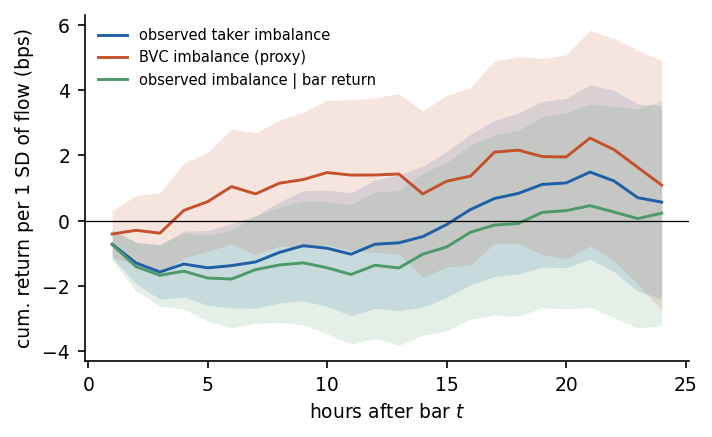
\includegraphics[width=0.7\textwidth]{fig_flow_response.png}
\caption{Cumulative log return (basis points) over $k$ hours following a one standard deviation flow
shock in hour $t$, from regression~\eqref{eq:response}, with 95\% Newey-West bands. Blue: observed
taker imbalance alone. Red: BVC imbalance alone. Green: observed imbalance holding the bar's
standardised return fixed. BTC/USDT.}
\label{fig:response}
\end{figure}

\begin{table}[t]
\centering\caption{Return response to order-flow shocks, BTC/USDT}\label{tab:response}
\begin{tabular}{lrrrrrr}
\toprule
Regressor (1 SD) & $k=1$h & $k=2$h & $k=4$h & $k=8$h & $k=12$h & $k=24$h\\
\midrule
Observed taker imbalance & \ensuremath{-}0.72 & \ensuremath{-}1.30 & \ensuremath{-}1.33 & \ensuremath{-}0.97 & \ensuremath{-}0.72 & 0.57\\
 & (\ensuremath{-}3.42) & (\ensuremath{-}3.99) & (\ensuremath{-}2.58) & (\ensuremath{-}1.23) & (\ensuremath{-}0.72) & (0.38)\\
BVC imbalance & \ensuremath{-}0.41 & \ensuremath{-}0.30 & 0.31 & 1.15 & 1.40 & 1.09\\
 & (\ensuremath{-}1.12) & (\ensuremath{-}0.55) & (0.42) & (1.17) & (1.16) & (0.56)\\
Observed imbalance, given $z_t$ & \ensuremath{-}0.73 & \ensuremath{-}1.41 & \ensuremath{-}1.55 & \ensuremath{-}1.36 & \ensuremath{-}1.37 & 0.23\\
 & (\ensuremath{-}2.97) & (\ensuremath{-}3.74) & (\ensuremath{-}2.61) & (\ensuremath{-}1.51) & (\ensuremath{-}1.20) & (0.13)\\
Bar return $z_t$, given imbalance & 0.02 & 0.26 & 0.50 & 0.89 & 1.48 & 0.78\\
 & (0.06) & (0.46) & (0.64) & (0.84) & (1.15) & (0.38)\\
\bottomrule
\end{tabular}

\tabnote{Coefficients from regression~\eqref{eq:response}: cumulative log return in basis points from
the close of hour $t$ to $t+k$ per one standard deviation of the regressor; Newey-West $t$-statistics
in parentheses. The third and fourth rows come from one regression with both regressors.}
\end{table}

Figure~\ref{fig:response} and Table~\ref{tab:response} show three facts. First, observed aggressor
flow predicts a \emph{reversal}. A one standard deviation increase in taker imbalance is followed by
a price decline of \BTCfrTakAone{} basis points over the next hour ($t=\BTCfrTakTone$) and \BTCfrTakAtwo{}
basis points over two hours ($t=\BTCfrTakTtwo$); the decline is \BTCfrTakAfour{} basis points at four
hours and has disappeared after about 15 hours. Buying pressure that is absorbed by passive orders is
followed by falling prices, which is consistent with a transient component of price impact
\citep{bouchaud2018} and with passive liquidity providers being, on average, on the right side of
the trade.

Second, the information is in the part of flow that the bar's price does not reveal. Holding the
standardised bar return fixed leaves the coefficient on observed imbalance essentially unchanged
(\BTCfrJointBtwo{} basis points at two hours, $t=\BTCfrJointTtwo$), while the bar return itself has no
predictive power ($t=\BTCfrZTtwo$ at two hours and $t=\BTCfrZTfour$ at four). Third, and as a
consequence, hourly BVC imbalance predicts nothing: its coefficient is \BTCfrBvcBtwo{} basis points at
two hours ($t=\BTCfrBvcTtwo$) and is positive, if insignificant, at longer horizons.
Section~\ref{sec:validation} showed that about three-quarters of the variance of observed imbalance
is invisible in the hourly bar's price change; this section shows that the invisible part is the part
that matters.

\paragraph{Controls and the best available proxy.} Table~\ref{tab:controls} asks whether the reversal
is a disguised return or volume effect. Adding three lags of the hourly return, 24-hour momentum,
standardised volume, volatility and the previous hour's imbalance leaves the two-hour coefficient at
\BTCrcctrlB{} basis points ($t=\BTCrcctrlT$). The flow effect is not a reversal of past returns and
not a volume or volatility effect. The last rows use the most accurate proxy we can build from price
data, BVC applied to one-minute bars and summed to the hour, whose correlation with observed
imbalance is \BTCbvcOneMinCorr{} rather than \BTCbvcCorr. On its own it does predict a reversal
(\BTCrcbvcmB{} basis points at two hours, $t=\BTCrcbvcmT$). When it competes with observed imbalance,
however, its coefficient falls to \BTCrcvsBvcmB{} ($t=\BTCrcvsBvcmT$) while observed imbalance keeps
\BTCrcvsTakB{} ($t=\BTCrcvsTakT$). Predictive content therefore rises with measurement accuracy: none
for hourly BVC, part of the signal for one-minute BVC, and all of it for observed flow, which subsumes
the proxy.

\begin{table}[t]
\centering\caption{Return response to observed flow with controls and against the best proxy}\label{tab:controls}
\resizebox{\textwidth}{!}{\begin{tabular}{lrrr}
\toprule
Specification (coefficient of interest) & $k=1$h & $k=2$h & $k=4$h\\
\midrule
\multicolumn{4}{l}{\emph{BTC/USDT}}\\
(1) taker & \ensuremath{-}0.72 (\ensuremath{-}3.4) & \ensuremath{-}1.30 (\ensuremath{-}4.0) & \ensuremath{-}1.33 (\ensuremath{-}2.6)\\
(2) + bar return & \ensuremath{-}0.73 (\ensuremath{-}3.0) & \ensuremath{-}1.41 (\ensuremath{-}3.7) & \ensuremath{-}1.55 (\ensuremath{-}2.6)\\
(3) + lagged returns, 24h momentum & \ensuremath{-}0.73 (\ensuremath{-}2.9) & \ensuremath{-}1.39 (\ensuremath{-}3.6) & \ensuremath{-}1.52 (\ensuremath{-}2.5)\\
(4) + volume, volatility, lagged taker & \ensuremath{-}0.64 (\ensuremath{-}2.5) & \ensuremath{-}1.32 (\ensuremath{-}3.7) & \ensuremath{-}1.52 (\ensuremath{-}2.8)\\
(5) 1m BVC alone & \ensuremath{-}0.65 (\ensuremath{-}2.4) & \ensuremath{-}1.00 (\ensuremath{-}2.5) & \ensuremath{-}0.75 (\ensuremath{-}1.3)\\
(6) taker vs 1m BVC: taker & \ensuremath{-}0.52 (\ensuremath{-}1.9) & \ensuremath{-}1.09 (\ensuremath{-}2.6) & \ensuremath{-}1.38 (\ensuremath{-}2.1)\\
(6) taker vs 1m BVC: 1m BVC & \ensuremath{-}0.33 (\ensuremath{-}1.0) & \ensuremath{-}0.35 (\ensuremath{-}0.7) & 0.09 (0.1)\\
\multicolumn{4}{l}{\emph{ETH/USDT}}\\
(1) taker & 0.10 (0.3) & \ensuremath{-}0.53 (\ensuremath{-}1.1) & 0.55 (0.8)\\
(2) + bar return & \ensuremath{-}0.15 (\ensuremath{-}0.4) & \ensuremath{-}0.79 (\ensuremath{-}1.5) & 0.21 (0.3)\\
(3) + lagged returns, 24h momentum & \ensuremath{-}0.13 (\ensuremath{-}0.4) & \ensuremath{-}0.75 (\ensuremath{-}1.4) & 0.24 (0.3)\\
(4) + volume, volatility, lagged taker & 0.00 (0.0) & \ensuremath{-}0.82 (\ensuremath{-}1.7) & 0.08 (0.1)\\
(5) 1m BVC alone & 0.33 (0.9) & \ensuremath{-}0.23 (\ensuremath{-}0.4) & 0.24 (0.3)\\
(6) taker vs 1m BVC: taker & \ensuremath{-}0.12 (\ensuremath{-}0.4) & \ensuremath{-}0.59 (\ensuremath{-}1.1) & 0.60 (0.7)\\
(6) taker vs 1m BVC: 1m BVC & 0.40 (0.9) & 0.10 (0.2) & \ensuremath{-}0.09 (\ensuremath{-}0.1)\\
\bottomrule
\end{tabular}
}
\tabnote{Coefficient (basis points per standard deviation) of observed taker imbalance, or of
one-minute BVC imbalance where indicated, in regressions of the $k$-hour return on standardised
regressors; Newey-West $t$-statistics in parentheses. (2) adds the standardised bar return; (3)
adds three lagged hourly returns and 24-hour momentum; (4) adds standardised volume, Garman-Klass
volatility and the previous hour's imbalance; (5) uses one-minute BVC imbalance alone; (6) includes
observed and one-minute BVC imbalance together.}
\end{table}

The magnitude is small. At four hours the observed-imbalance regression explains
\BTCfrRtwoFour\% of the return variance, and the implied move of one to two basis points per standard
deviation compares with a standard spot fee of ten basis points per side. Even a perfect measurement
of flow at this frequency would therefore be of little direct use for trading, a conclusion the next
section confirms out of sample.
